\chapter{Design di dettaglio}\label{ch:design-di-dettaglio}

\section{Lista di componenti}\label{sec:lista-di-componenti}
Una caratteristica importante della libreria è permettere di specificare nel tipo di un sistema (o una view)
su quali componenti questi operano, così che le stesse firme dei metodi possano guidare il programmatore indicando i
tipi dei componenti trattati.
Così facendo si elimina la necessità di specificare a tempo di esecuzione il tipo di componenti richiesto (come per
esempio è necessario fare nella libreria Ashely~\cite{ashley} che ricorre al passaggio di oggetti \texttt{Class<?>})
permettendo di intercettare diversi errori a tempo di compilazione.

Realizzare tale funzionalità a livello di compilazione si è rivelato essere una sfida che ha richiesto l’implementazione
delle \texttt{CList}, nonché l’utilizzo di macro per modificare il comportamento del compilatore introducendo controlli
personalizzati (descritti in~\ref{subsec:macro}).

Una \texttt{CList} (abbreviazione di Components List) è essenzialmente una lista di elementi eterogenei che preserva
informazioni sul tipo di ciascun elemento in maniera simile a una tupla.
Per esempio si osservi il Listato~\ref{lst:lstinputlisting2}: la lista che contiene
i componenti Position e Velocity avrà come tipo~\texttt{Position~\&:~Velocity~\&:~CNil}, permettendo di conoscere il
tipo e la posizione dei suoi elementi.

Nel Listato~\ref{lst:lstinputlisting2} viene mostrato un esempio di utilizzo delle \texttt{CList} nelle~\texttt{View}.
\lstinputlisting[label={lst:lstinputlisting2}, caption=Esempio di utilizzo delle CList.]{code/clist-usage.scala}

L’idea alla base di questa soluzione è ispirata dalle Heterogeneous List della libreria
Shapeless\cite{shapeless}; una differenza significativa sta nel fatto che la definizione di una \texttt{CList} impone un
limite ulteriore sul tipo dei suoi elementi: devono tutti essere sottotipi di \Component, parte dell’implementazione è
riportata al Listato~\ref{lst:lstinputlisting}.

\lstinputlisting[label={lst:lstinputlisting}, caption=Esempio di codice per implementare CList.]{code/clist.scala}

\section{Container dei componenti}\label{sec:container-dei-componenti}
\section{Builder dei sistemi}\label{sec:builder-dei-sistemi}
\section{DSL}\label{sec:dsl}

\begin{figure}
    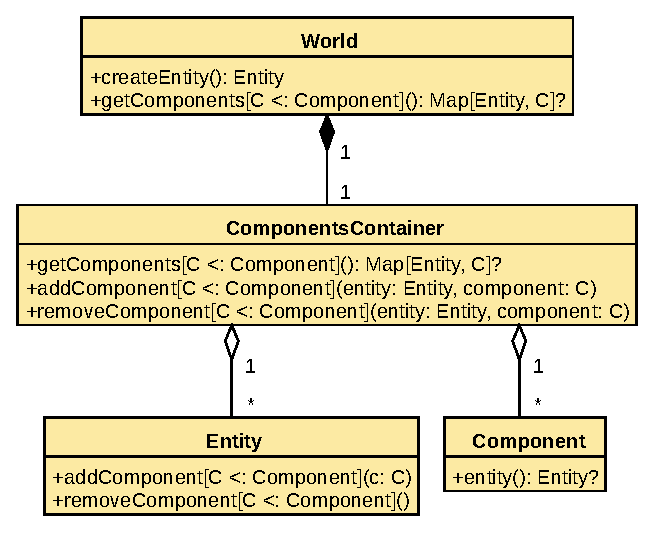
\includegraphics{./img/WorldDetail}
    \caption{Design di dettaglio}
    \label{fig:figure2}
\end{figure}